\makeatletter
\def\input@path{{../../}}
\makeatother
\documentclass[../../main.tex]{subfiles}
\graphicspath{
	{../../img/}
	{../img/}
	{img/}
}

\begin{document}
В общем случае если имеется окружность радиуса $R$ с центром в точке $O$ и
две точки $M$ внутри, 1а  $N$ вне окружности то, проводя луч $OMN$, говорят,
что точки $M$ и $N$ находятся в \emph{инверсии(симметрии)} отностительно
рассматриваемой окружности, если $OM \cdot ON = R^2$.

Для простейшего $ w = \frac{1}{z}$  имеем: 
$ |w| = \frac{1}{|z|} \implies |z| \cdot |w| = 1 $ т.~е. преобразование $z$
и из плоскости \textcircled{$z$}  и образ $w$ в  \textcircled{$w$} будут
находиться в инверсии относительно окружности с $R  = 1$.

\begin{center}
	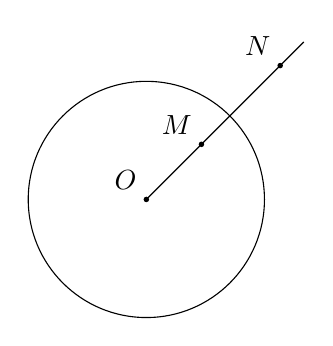
\begin{tikzpicture}
    \draw[color=black] (0,0) circle(1.5);
    \fill(0,0) circle(1pt) node[above left] {$O$};
    \fill(0.7,0.7) circle(1pt) node[above left] {$M$};
    \fill(1.7,1.7) circle(1pt) node[above left] {$N$};
    \draw (0,0) -- (2,2);
	\end{tikzpicture}
	\begin{tikzpicture}
	\draw[->] (-2.5,0) -- (2.5,0);
	\draw[->] (0,-2.5) -- (0,2.5) node[below right] {\textcircled{$z$}};
    \draw[loosely dashed] (0,0) circle(1.5);
    \draw(1.5, -0.1) node[below left]{$1$}-- (1.5, 0.1);
    \draw(-1.5, -0.1) node[below left]{$-1$} -- (-1.5, 0.1);
    \fill(0.6,0.6) circle(1pt) node[above left] {$Z$};
	\end{tikzpicture}
	\begin{tikzpicture}
	\draw[->] (-2.5,0) -- (2.5,0);
	\draw[->] (0,-2.5) -- (0,2.5) node[below right] {\textcircled{$w$}};
    \draw[loosely dashed] (0,0) circle(1.5);
    \draw(1.5, -0.1) node[below left]{$1$}-- (1.5, 0.1);
    \draw(-1.5, -0.1) node[below left]{$-1$} -- (-1.5, 0.1);
    \fill(0,0) circle(1pt) node[above left] {$O$};
    \fill(0.7,0.7) circle(1pt) node[above left] {$M$};
    \fill(1.7,1.7) circle(1pt) node[above left] {$N$};
    \draw (1.9,1.5) node[right]  {$w = \frac{1}{z}$};
    \draw (2,0.6) node[right]  {$OM \cdot ON = 1$};
    \draw (0,0) -- (2,2);
	\end{tikzpicture}
\end{center}
В дальнейшем под \emph{окружностью(прямой)} на КП в широком смысле слова будем
подразумевать, как \emph{окружность}, так и \emph{прямую}.
В соответствии с этим общее дробно-линейным пребразованием обладает следующим
свойством: \emph{окружнсоть} при дробно-линейном преобразовании переходит либо
в \emph{окружность}, либо в \emph{прямую}, а \emph{прямая} может перейти как
в \emph{прямую}, так и в \emph{окружность}.

т.~к. \emph{линейное отображение}
является частным случаем \emph{дробно-линейного}, то для него существет
подобное свойство: \emph{прямая} переходит только в \emph{прямую},
\emph{окружность} ~-- только в \emph{окружность}.

Если в плоскости \textcircled{$z$} заданы различные точки $z_1, z_2, z_3$
переходящие при соответствующем дробно-линейном преобразовании 
\eqref{lec25:7} переходят последовательно в точки $w_1, w_2, w_3$ в 
\textcircled{$w$}, то можно показать что \eqref{lec25:7} в этом случае
удавлетворяет условию:
\begin{equation}
\label{lec26:1} \frac{w - w_1}{w - w_2} \cdot \frac{w_3 - w_2}{w_3 - w_1} = 
\frac{z - z_1}{z - z_2} \cdot \frac{z_3 - z_2}{z_3 - z_1}
\end{equation}

В случае, когда рассматриваемая КП и \eqref{lec26:1} одна из т.
$z_k , k = \overline{1,3}$ или $w_k , k = \overline{1,3}$ равна 
$\infty$, то тогда все разности в \eqref{lec26:1}, испльзующие 
эти точки, делим на $1$.

Например, если $z_3 = \infty \implies w_3 \neq \infty$ 
\eqref{lec26:1} $(\rightarrowtail)$
\[
\frac{w - w_1}{w - w_2} \cdot \frac{w_3 - w_2}{w_3 - w_1} = 
\frac{z - z_1}{z - z_2}
\]
Аналогично, если 
$z_3 = \infty \underset{\text{переходит в}}{\rightarrowtail} w_3 = \infty$
\[
\frac{w - w_1}{w - w_2} = \frac{z - z_1}{z - z_2}
\]

\begin{examples}\
 \begin{enumerate}
  \item
 Найдём дробно-линейное преобразование \eqref{lec25:7}, 
 для которого
 \[
 \begin{cases}
w(1) = i \\ 
w(0) = 2 \\
w(i) = 1  
 \end{cases}
\]
 \[
  z_1 = 1 \rightarrowtail w_1 = i
  z_2 = 0 \rightarrowtail w_1 = 2
  z_3 = i \rightarrowtail w_1 = 1
 \]
 т.~к. $z_1, z_2, z_3$ не лежат на одной прямой в \textcircled{$z$}, 
 а $w_1, w_2, w_3$ также не лежат на одной прямой в \textcircled{$w$}
 $\implies$ окружность плоскости \textcircled{$z$} проходящая через
 $z_1, z_2, z_3$  перейдёт в соответствующую окружность \textcircled{$w$},
 проходящую через $w_1, w_2, w_3$. В силу \eqref{lec26:1}:
 \[
  \frac{1 - 2}{1 - i} \cdot \frac{w - i}{w - 2} = 
  \frac{z - 1}{z - 0} \cdot \frac{-i - 0}{-i - 1} =
  \frac{z - 1}{z} \cdot \frac{1}{1 - i}
 \]
 \[
  -\frac{w - i}{w - 2} = \frac{z - 1}{z}
 \]
 \[
  -zw +iz = (z - 1)(w - 2) = zw - 2z - w + 2
 \]
 \[
  (2z - 1)w = (2 + i_z + 2
 \]
 \[
  w = \frac{(2 + i) + 2}{2z - 1}
 \]
\[
 z= \frac{1}{2} \rightarrowtail w = \infty
\]
\item
\[
 \begin{cases}
  w(0) = \infty\\
  w(\infty) = i\\
  w(1 + i) = 1 + i
 \end{cases}
\]
В этом случаем, в силу \eqref{lec26:1} имеем:
\[
  \begin{cases}
  w(0) = \infty\\
  w(\infty) = i\\
  w(1 + i) = 1 + i
 \end{cases}
 \implies \frac{w_3 - w_2}{w - w_2} = \frac{z - z_1}{z_3 - z_1}
\]
\[
 \frac{1 + i - i}{w - i} = \frac{z - 0}{1 + i - 0} \implies
 w - i = \frac{1 + i}{z} \iff w = \frac{1 + i}{z} + i
\]
Можно показать, что имеют место слудующие частные случаи 
дробно-линейных отображений:
\begin{enumerate}
 \item 
 \[
  \begin{cases}
   w = A \frac{z - z_1}{z - z_2} \\
   A \in \C
  \end{cases}
  \text{При этом}
\begin{cases}
  z_1 \rightarrowtail 0 \\
  z_1 \rightarrowtail 0   
 \end{cases}
 \]
Если окружность(прямая) содержит точку $z_2$, то при рассмотрении отображения
её образом будет прямая, иначе -- окружность.
 \item
\[
\begin{cases}
 w = e^{i\alpha} \frac{z - z_0}{z- \overline{z_0}} \\
 \alpha \in \R,  \operatorname{Im} z_0 > 0
\end{cases}     
\]
При этом отображении 
\[
\operatorname{Im} z_0 > 0\,  \text{\textcircled{$z$}}
\]
\[
|w| < 1\,  \text{\textcircled{$w$}}
\]
т. $z_0$ из \textcircled{$z$} переходит в центр круга плосскости
\textcircled{$w$}.

 \item
\[
 \begin{cases}
  w = e^{i\alpha} \frac{z - z_0}{1 - z \overline{z}} \\
  \alpha \in \R
 \end{cases}
\]
При этом отображении единственный круг в плоскости \textcircled{$z$}
переходит в единственный круг \textcircled{$w$} так, что т. $z_0$ переходит
в центр круга  $w_0$ в пл. \textcircled{$w$}.


\end{enumerate}

\end{enumerate}
\end{examples}

\section{Степенная ФКП с натуральным показателем и обратной к ней ФКП}
Рассмотрим
\begin{equation}
\label{lec26:2}
\begin{cases}
 w = f(z) = z^n \\
 n \in \N
\end{cases}
\end{equation}

Если $n = 1$, то $w \stackrel{\eqref{lec26:2}}{=} z$ ~-- 
идентичное ФКП(отображение) \\
При этом отображение и преобразование плоскости \textcircled{$z$} 
даёт такой же образ \textcircled{$w$}. \\
Пусть $n \geq 2$
\[
\begin{cases}
 z =re^{i\phi} \qquad\qquad\qquad\qquad 
 w\stackrel{\eqref{lec26:2}}{=} r^ne^{in\phi}\\
 r = |z| \\
 \phi = \operatorname{arg} z \in \left] -\pi, \pi \right] \implies 
 \begin{cases}
 |w| = r^{n} \\
 \operatorname{Arg}w = n \phi + 2\pi k, k \in \Z
 \end{cases}
\end{cases}
\]

Рассмотрим частныйы случай $n = 2$, т.~е. $w = z^2 = r^2e^{2i\phi}$
\[
 \begin{cases}
  |w| = r^2 \\
\operatorname{Arg} w = 2\phi + 2\pi k, k \in X
 \end{cases}
\]
\begin{enumerate}
\item
\[
0 < \operatorname{arg} z < \frac{\pi}{2} \implies 
\phi =\operatorname{Arg} w = \pi + 2 \pi k, k \in \Z
\]
$I$ ~-- я четверть \textcircled{$z$} $\longrightarrow$ 
верхняя полуплоскость плоскости \textcircled{$w$}.
\begin{center}
	\begin{tikzpicture}
	\draw[->] (-2.5,0) -- (2.5,0);
	\draw[->] (0,-2.5) -- (0,2.5) node[above right] {\textcircled{$z$}};
	
    \pattern[pattern=north east lines] 
    (0.3,0.3)--(0.3,2.5)--(2.5,2.5)--(2.5,0.3)--cycle;
    \draw[dashed] (0.3,0.3) -- (0.3,2.5);
    \draw[dashed] (0.3,0.3) -- (2.5,0.3);
	
    \draw[->] (4.5,0) -- (9.5,0);
	\draw[->] (7,-2.5) -- (7,2.5) node[above right] {\textcircled{$w$}};
	
    \pattern[pattern=north east lines] 
    (4.5,0.3)--(9.5,0.3)--(9.5,2.5)--(4.5,2.5)--cycle;
    \draw[dashed] (4.5,0.3) -- (9.5,0.3);
    
    \draw[->, thick] (2.6,2) .. controls (3.5,2.5) .. (4.4, 2)
    node[pos=0.6,above]{$w = z^2$};
	\end{tikzpicture}
\end{center}

\item
\[
 0 < \operatorname{arg} z < \pi \implies \phi = 2\pi + 2\pi k, k \in \Z
\]
В данном случае верняя полуплоскость \textcircled{$z$}
$\longrightarrow$ во всю плоскость  \textcircled{$w$}
c разделением вдоль положительной части действительной оси.

\begin{center}
	\begin{tikzpicture}
	\draw[->] (-2.5,0) -- (2.5,0);
	\draw[->] (0,-2.5) -- (0,2.5) node[above right] {\textcircled{$z$}};
	
    \pattern[pattern=north east lines]
    (0.3,0.3)--(0.3,2.5)--(2.5,2.5)--(2.5,0.3)--cycle;
    \draw[dashed] (0.3,0.3) -- (0.3,2.5);
    \draw[dashed] (0.3,0.3) -- (2.5,0.3);
	
    \draw[->] (4.5,0) -- (9.5,0);
	\draw[->] (7,-2.5) -- (7,2.5) node[above right] {\textcircled{$w$}};
	
    \pattern[pattern=north east lines]
    (4.5,0.3)--(9.5,0.3)--(9.5,2.5)--(4.5,2.5)--cycle;
    \draw[dashed] (4.5,0.3) -- (9.5,0.3);
    \pattern[pattern=north east lines]
    (4.5,-0.3)--(9.5,-0.3)--(9.5,-2.5)--(4.5,-2.5)--cycle;
    \draw[dashed] (4.5, -0.3) -- (9.5, -0.3);
    
    \draw[->, thick] (2.6,2) .. controls (3.5,2.5) .. (4.4, 2)
    node[pos=0.6,above]{$w = z^2$};
	\end{tikzpicture}
\end{center}
\end{enumerate}

Аналогично поступают и в слуачях: $n \in \N, n \geq 2$.
Обратную к степенной функции с натуральным показателем $n \in \N: w^n = z$
определяют как решение уравнения: 
$w = {|z|}^{\frac{1}{n}e^{i\operatorname{arg}\frac{z + 2 \pi k}{n}}}$ 
$\implies$ многозначность, если придавать $k \in \Z$ последовательно
значения, то последнее из них будет двавать одну из ветвей рассмотренной
многозначной ФКП. На практике для определения ветви рассматривают 
соответствующие начальные условия 
$(z_0 \neq 0)\; \sqrt{z_0} = {|z|}^{\frac{1}{n}}e^{i
\frac{\phi + 2 \pi m}{n}}, m \in \Z$, где по значению 
$\sqrt[n]{z}$ однозначно ??? $m \in \Z$ $\implies$ для найденного 
$m \implies w = \sqrt[n]{z} = |z|^{\frac{1}{n} 
e^{i \frac{\phi_0 + 2 \pi k}{n}}}$.


\begin{example}
 Рассмотрим ветвь $\sqrt[3]{z}$, для которой 
 $\sqrt[3]{i} = e ^{i \frac{\pi}{6}}$. В данном случае для 
 $z_0 = i \implies z_0 = |z_0| e^{i(\phi_0 + 2 \pi k)} = 
 e^{i(\frac{\pi}{2} + 2 \pi k)} \implies \sqrt[3]{z} = 
 (e^{i(\frac{/pi}{2} + 2 \pi k)})^{\frac{1}{3}} =
 e^{i(\frac{\pi}{6} + \frac{2 \pi k}{3})}$ \\
 т.~к. в слиу начального условия 
 $\sqrt[3]{i} = e ^{i \frac{\pi}{6}}$, то 
 $k = 0 \implies m = \frac{2 \pi k }{3} = 0$, 
 поэтом в данном случае $w = \sqrt[3]{z}
 = {|z|}^{\frac{1}{3}}e ^{i( \frac{\pi}{6} + 0)}
 = {|z|}^{\frac{1}{3}}e ^{i( \frac{\pi}{6})} 
 = \frac{sqrt{3} + i }{2} \sqrt[3]{|z|}$
\end{example}

\subsection{Комплексная экпонента. Гиперболические и тригонометрические ФКП}
Для 
$
\begin{cases}
 z = x + iy \\
 x, y \in \R
\end{cases}
$
по определению $\exp{z} = e^x(\cos x + i \sin y) $ \\
Если $y = \operatorname{Im} z = 0$, то $z = x \in \R$ \\
$\exp z = e^x$
В дальнейшем в общем случае будем использовать
\begin{equation}
\label{lec26:3}
 \exp{z} = e^z = e^{x + iy} = e^{x}(\cos x + i \sin x)
\end{equation}
В силу \eqref{lec26:3} имеем:
 \begin{enumerate}
    \item $e^0 = 1$
    \item $^{z_1} \cdot e^{z_2} = e^{z_1 + z_2}, \forall z_1, z_2 \in \C$
    \item $\frac{e^{z_1}}{e^{z_2}} = e^{z_1 - z_2}, \forall z_1, z_2 \in \C$
 \end{enumerate}
В отличии от действ $\exp$, $\exp$ \eqref{lec26:3} будет 
периодическоей ФКП с основным периодом $T_0 = 2\pi i$, т.~к.
$\forall k \in \Z \implies e^{z + 2 T_0} = e^{z + 2 \pi k i} 
= e^{z} e^{2 \pi k i} = e^z(\cos{2 \pi k} + i \sin{2 \pi k}) = e^z$

С помощью \eqref{lec26:3} определяют гиперболические ФКП
\[
 \ch{z} = \frac{e^z + e^{-z}}{2}
\]
\[
 \sh{z} = \frac{e^z - e^{-z}}{2}
\]
\[
 \th{z} = \frac{\sh{z}}{\ch{z}} = \frac{e^{2z} - 1}{e^{2z} + 1}
\]
\[
 z \neq i(\frac{\pi}{2} + \pi k), k \in \Z
\]
\[
 \cth{z} = \frac{\ch{z}}{\sh{z}} =
 \frac{e^{2z} + 1}{e^{2z} - 1}, z \neq i \pi k, k \in \Z
\]
Для гиперболеческой ФКП сохраняется свойство действительности
Например:
\begin{enumerate}
 \item $\ch^{2}{z} - \sh^{2}{z} = 1$  ~-- основное гиперболическое тождество
 \item $1 - \th^{2}{z} = \frac{1}{\ch^{2}{z}}$
 \item $\cth^{2}{z} - 1= \frac{1}{\sh^{2}{z}}$
 \item $\sh{2z} = 2\sh{z} \ch{z}$
 \item $\ch{2z} = \ch^{2}{z} + \sh^{2}{z}$
\end{enumerate}

В отличие от тригонометрического $\sin$ и $\cos$, которые являются 
ограниченными, гиперболические ФКП не обязательно будут ограничены.\\
Полагаем $\cos{z} = \frac{e^{iz} + e^{-iz}}{2} = \ch{iz}$
\[
 \sin{z} = \frac{e^{iz} - e^{-iz}}{2i} = -i \sh{iz}
\]

\[
 \tg{z} = \frac{\sin{z}}{\cos{z}}, z \neq \frac{\pi}{2} k, k \in \Z
\]
\[
 \ctg{z} = \frac{\cos{z}}{\sin{z}}, z \neq \pi k, k \in \Z
\]
А также:
\[
 \cos^2{z} + \sin^2{z} = 1
\]
\[
 1 + \tg^{2}{z} = \frac{1}{\cos^2{z}}
\]
\[
 1 + \ctg^{2}{z} = \frac{1}{\sin^2{z}}
\]
\[
 \sin{2z} = 2 \sin{z} \cos{z}
\]
\[
 \cos{2z} = \cos^{2}{z} -  \sin^{2}{z}
\]

Хотя для тригонометрических ФКП выполняется основные тригонометрические
тождества(О.Т.Т),но из него уже не следует ограниченность 
тригонометрической ФКП.

\subsection{Логарифмичсекая ФКП}
Логарифмичсекая ФКП обозначается $w = \operatorname{Ln}{z}$ 
и определяется как решение уравнения 
\begin{equation}
 \label{lec26;4}
 \begin{cases}
   e^{2} = z \\
   z \neq 0
 \end{cases}
\end{equation}

 

\end{document}
